% !TEX root = ../../main.tex
\section{Change Detection}\label{sec:method_change_detection}
In the previous sections we have discussed what data is used for the model construction, and how that model is interpreted in the context of change detection.
We have shown how the multi-dimensional signal is reduced to a single dimension time series data, based on the extracted radius $R$ from the constructed hypersphere.
This metric is used to discover changes in the underlying data generation process.
We argued that in the case the data objects set becomes more heterogeneous, we expect an increase in the radius $R$.
In the same manner we expect that when the change is in the oldest data objects of the working set, the radius $R$ will decrease, since the data becomes more homogeneous.
An abstract representation of these expectations is illustrated in \Cref{fig:radius_expectation}.

In this section we discuss the methods applicable to the extracted radius $R$ of the hypersphere, in order to discover a change in the underlying distribution properties.
It is the second stage of our algorithm, analogue to the second stage of the unifying framework by Takeuchi and Yamanishi~\cite{takeuchi2006unifying}.
It is also based on the \gls{svcpd} method by Camci~\cite{camci2010change}, although we have simplified the algorithm.

\begin{table}
\begin{center}
  \caption[Proposed algorithm]{Algorithm of the proposed change detection method, using the Ratio-Thresholding method of \ref{subsec:ratio_thresholding} for change detection.}
  \begin{tabular}{ l p{12cm} }
    \hline
    Step & Action \\
    \hline
    & \textbf{Input:} time series $\vectorsym{x}$, window size $n$ \\
    & \textbf{Output:} collection of change points $\vectorsym{t}$ \\
    1 & Start with $n$ data objects as working set and construct hypersphere \\
    2 & Add next data object $x_t$ and drop first one \\
    3 & Identify new hyper-sphere and its \emph{approximate radius} \\
    4 & Calculate radius average of hyperspheres since last change point \\
    5 & Calculate radius ratio $\hbar$. \newline
    If $\hbar$ is  lower than ${th}_{low}$ or greater than ${th}_{high}$ then mark $t$ as change point in $\vectorsym{t}$ \\
    6 & Continue from step 2, until no more data objects available \\
    7 & Apply post-processing: merge close change points \\
    \hline
  \end{tabular}
  \label{tab:algorithm_proposed_method}
\end{center}
\end{table}

\TODO{Algoritme meer in pseudo-code zetten. Prominenter maken.}


\begin{algorithm}
\caption{\acrlong{ocs-hats} algorithm.}
\label{alg:ocs-hats}
\begin{algorithmic}[1]
\Require time series $\vectorsym{x}$ and window size $n$
\Ensure collection of change points $\vectorsym{cp}$

\State $w \leftarrow \vectorsym{x}[1 \dots n-1]$ \Comment{Initialize working set}

\While{$\vectorsym{x}_t$ is available}
  \State $w[] \leftarrow \vectorsym{x}_t$ \Comment{Add new data to working set}

  \State $s \leftarrow \operatorname*{SVDD}(\vectorsym{x})$ \Comment{Create hypersphere with SVDD method}
  \State $r[] \leftarrow s.radius$ \Comment{Extract radius from hypersphere}

  \State $r_{avg} \leftarrow \operatorname*{average}(r)$
  \State $\hbar \leftarrow s.radius / r_{avg}$ \Comment{Radius ratio $\hbar$}

  \If{ $\hbar$ \textless $th_{low}$ \textbf{or} $\hbar$ \textgreater $th_{high}$} \Comment{Compare $\hbar$ with thresholds}
    \State $cp[] \leftarrow t$ \Comment{Mark $t$ as change point}
  \EndIf

  \State $w[0] \leftarrow []$ \Comment{Drop oldest data point from working set}
\EndWhile

\State $cp \leftarrow \operatorname*{merge}(cp)$ \Comment {Post-processing, change point merging}
\end{algorithmic}
\end{algorithm}

\TODO{Make algorithm more readable}

In the \gls{svcpd} the first step for a new data point $\vectorsym{z}$ is to check whether the data point lies within the enclosing (hyperspherical) boundary of the constructed model.
This will label the new data point as an in- or outlier, relative to the current data set.
Depending on that outcome, the model is updated to include the new data point.
The second step is to inspect the (changed) model properties, \ie the radius $R$.
In \gls{ocs-hats} we only employ the second step: the inspection of the radius $R$.
We regard the first step (determine if $\vectorsym{z}$ is an outlier) to be superfluent: in case it is an outlier, the model update step will change the radius $R$ in order to let the boundary include the new data point $\vectorsym{z}$.
Would the new data object $\vectorsym{z}$ be already an inlier, then the updated model would not have a significant change in radius $R$.
Our algorithm is outlined in \Cref{tab:algorithm_proposed_method}.

The problem of change detection in complex multi-dimensional time series is now reduced to finding change in a one-dimensional time series.
Besides the dimensionality reduction, the form of the signal is also simplified.
Whereas the original signal was represented as a sinusoidal or second order \gls{ar} model, the new time series is of much simpler form.
In our method we leave open the precise method which is used to find change points in the obtained change indication values.
Below, we will gives two examples of methods which can be applied.
The first is a family of methods based on the \gls{cusum} method.
The second example is a ratio-based thresholding mechanism used by Camci~\cite{camci2010change}.
We conclude this section by discussing some post-processing techniques we have used, to decrease the number of false positives.

\subsection{CUSUM based methods}
Many of the simple change detection methods are based on \gls{cusum}, originally introduced by Page~\cite{page1954continuous}.
Other variations and extensions of the method are proposed and used (\cite{inclan1994use,alippi2006adaptive,hsu2007mosum}).
Here we will discuss the simple form, which only detects changes as an increase in value of the examples, in this case the radius $R$.
The cumulative sum for all the values is calculated:
\begin{equation}
  S_n = \sum_{k=0}^n R_k
\end{equation}
and a change is detected when the value of the cumulative sums minus the minimum encountered exceeds a predetermined threshold $h$:
\begin{equation}
  \left\{ S_n - \operatorname*{min}_{0 \le i < n} S_i \right\} \ge h.
\end{equation}

Extensions of the \gls{cusum} method have been proposed.
Amongst others, extensions which extend its use to two-threshold methods, and methods appropriate for changes in mean or variance \cite{inclan1994use}.
Whilst adaptive methods have been proposed \cite{alippi2006adaptive}, most methods require manual determination of the threshold parameter $h$.

\subsection{Ratio-thresholding}\label{subsec:ratio_thresholding}
The second example of an algorithm that interprets the change indication time series and transforms it to change detection is the radius ratio thresholding method used by Camci~\cite{camci2010change}.
The method shares characteristics with \gls{cusum}, since it relies on summation of historic data and thresholds for change detection.
The method calculates the radius ratio $\hbar_t$ by taking the ratio of the current radius $r_t$ at time $t$ to the average radii since the last change point $y$:
\begin{equation}\label{eq:ratio_radius}
  \hbar_t = \frac{r_t}{\operatorname*{mean}(r_{y:t-1})},
\end{equation}
where $\operatorname*{mean}(r_{y:t-1})$ is the average of the previous approximated radii.
By using only historic data, this method can be incorporated in an online change detection method.
The ratio $\hbar_t$ is compared with two thresholds: the low threshold $th_\text{low}$ and the high threshold $th_\text{high}$.
When the data objects in the working set become more homogeneous at time $t$, the radius $R$ of the hypersphere and thereby the ratio $\hbar_t$ will decrease.
When the new value of $\hbar_r$ is lower than the low threshold $th_\text{low}$, a change detection is observed for time $t$.
The same holds for a more heterogeneous set of data and an increase of $\hbar_r$ higher than $th_\text{high}$.
This is illustrated in \Cref{fig:tresholding}.

The appropriate values for the thresholds strongly depend on the characteristics of the data and the parameter $C$ (as discussed in \Cref{subsec:oc-svm-svdd}).
This trade-off parameter regulates the fraction of data objects that will be rejected from the constructed model.
Since a high value of $C$ assigns a high penalty to outliers, data objects are more likely to be incorporated into the hypersphere by increasing the radius.
For low values of $C$ the cost of rejecting data objects is, compared to the benefits of a smaller hypersphere, relatively low.
This gives a relation between the parameters $C$, $th_\text{low}$, $th_\text{high}$, and the sensitivity of the radius ratio based thresholding method.
A high value of $C$, or values close to $1$ for $th_\text{low}$ and $th_\text{high}$ result in a sensitive change detection procedure.
The reverse results in less sensitive methods.
The correct values for the intended sensitivity need to be empirically determined.

\begin{figure}
  \centering
    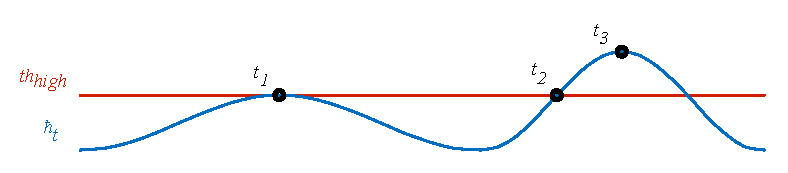
\includegraphics[width=\textwidth,height=\textheight,keepaspectratio]{./Figures/chapter4/signal_threshold.pdf}
  \caption[Thresholding]{Abstract illustration of the radius ratio thresholding. The peak at $t_1$ generates a single change point. The region between $t_2$ and $t_3$ generates multiple change points, since the value of $\hbar_t$ keeps increasing.}
  \label{fig:tresholding}
\end{figure}

\subsection{Post-processing}
In our method we use the ratio based thresholding, also used by Camci~\cite{camci2010change}.
From preliminary experiments we observed that a single change in the data can cause many detected change points, using the ratio based method.
This phenomenon can be explained by the nature of the thresholding method.
Since a single (high or low) threshold is set for ratio of the radii, high values are considered to be a change point before the highest point of the peak.
As illustrated in \Cref{fig:tresholding}, the peak at $t_1$ represents a single change point.
The region from $t_2$ to $t_3$ is strictly increasing.
At $t_2$ a change point is detected, since $\hbar_t$ exceeds the threshold.
But since it is increasing up to $t_3$, all values of $\hbar_t$ in that period will trigger the ratio based method to indicate a change point.

To overcome this problem, we apply a post-processing method on the generated change points.
All the change points that are within a time period $\delta$ of each other are merged together.

In the following two chapters we will take a detailed look at the used data sets and apply the method as described in this method to those sets.